\documentclass[12pt, a4paper]{article}

% --- Paquetes básicos ---
\usepackage[utf8]{inputenc}
\usepackage[spanish]{babel}
\usepackage[margin=2.5cm]{geometry}
\usepackage{graphicx}
\usepackage{float}
\usepackage{amsmath, amssymb}
\usepackage{fancyhdr}

% --- Configuración del Título ---
\title{Bloque 2: Simulación de Carga de Trabajo y Monitorización}
\author{Juan Reche Aguilar}
\date{\today}

% --- Configuración de Encabezados ---
\pagestyle{fancy}
\fancyhf{}
\rhead{Ingeniería de Servidores}
\lhead{Juan Reche Aguilar}
\cfoot{\thepage}

\begin{document}

\maketitle

\tableofcontents
\newpage

\section{ Ejercicio 4.3.1. Logs de arranque del sistema. }

\begin{figure}[H]
    \centering

    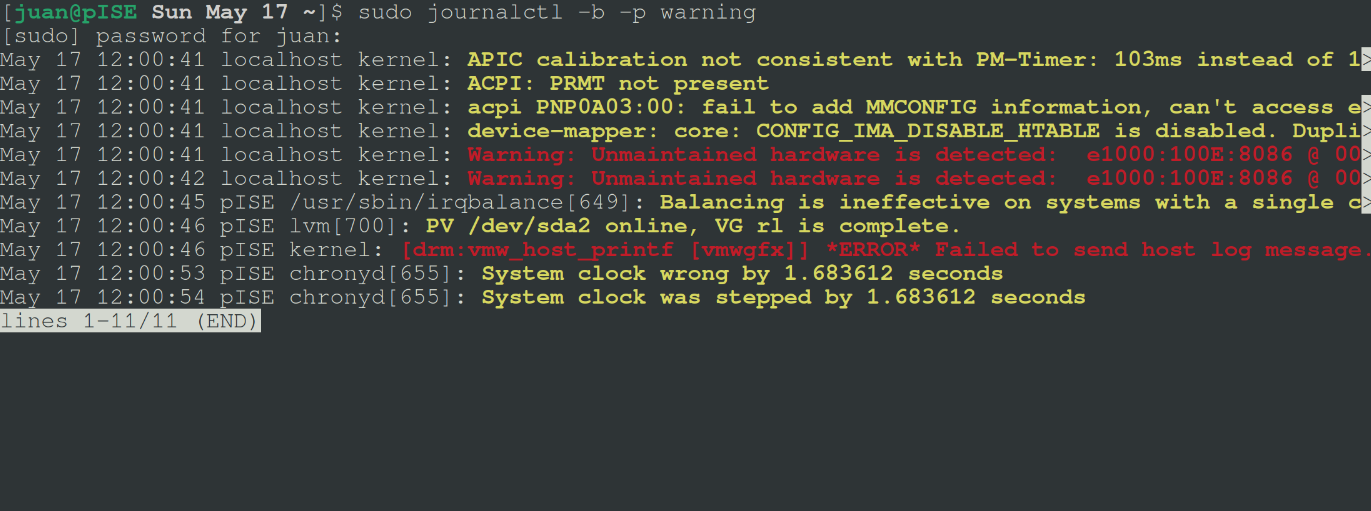
\includegraphics[width=1\textwidth]{../../capturas4/seccion3/comando.png}

    \caption{Ejecucion del comando journalctl.}

\end{figure}

La opcion -b se utiliza para mostrar los mensajes del arranque actual del sistema.
La opcion -p warning se utiliza para filtrar los mensajes y mostrar solo aquellos que 
tienen un nivel de prioridad de "warning" o superior.

\end{document}